\documentclass[12pt]{article}
\usepackage[T1]{fontenc}
\usepackage[utf8]{inputenc}
\usepackage{lmodern}
\usepackage{indentfirst}
\usepackage[bookmarks, colorlinks=true, linkcolor=black, citecolor=black, urlcolor=blue]{hyperref}
\usepackage{amsmath}
\usepackage{hyperref}
\usepackage{hyphenat}
\usepackage{graphicx}
\usepackage[a4paper]{geometry}
\usepackage[magyar]{babel}
\author{Endreffy Zsolt}
\title{Near Field Communication}

\begin{document}

\maketitle

\pagebreak

\tableofcontents

\pagebreak

\section{Bevezetés}
Napjainkban egyre többször lehet találkozni a legkülönfélébb alkalmazási 
területeken a \emph{Near Field Communication}-nel, avagy az \emph{NFC}-vel.
Főként mobiltelefonokba beépítve nyer egyre nagyobb teret ez a technológia,
hiszen itt tudják a szolgáltatók a technológiát (fizetős) szolgáltatásokkal
összekötni.

De mi is ez a technológia, és hogyan is működik?
Ebben a munkában ezt a kérdést szeretném körbejárni, kezdve egy rövid 
elméleti összefoglalóval, ezt folytatva a technikai paraméterek leírásával,
szót ejtve az NFC biztonsági vonásairól. Végül két másik vezeték nélküli
technológiával is összevetem, hogy könnyebb legyen elhelyezni ezt a 
feltörekvő technológiát.

\section{A közeltér-távoltér különbségéről}

\subsection{A régiók rövid összefoglalása}
Ahogy a közeltér neve is sugallja, elsősorban az antennához közeli távolságban
beszélhetünk róla, míg távoltér esetén értelemszerűen a messzebb eső 
távolságokban. A kettő határa azonban nincs konkrétan megszabva, mert az
függ még a forrás által sugárzott domináns hullámhossztól is.

Ha megvizsgáljuk a Hertz-dipólusra, mint elemi antennára felírható egyenleteket,
akkor sok hasznos tanulságot levonhatunk a közel- és távoltér különbségéről.

A gömbkoordináta rendszerben kifejezett $\mathbf{E}$ és $\mathbf{H}$ térerősségek
\cite[177.~oldal]{elektromagnesesterek}:

\begin{equation}
H_{\phi} =  \frac{I_0 l}{4 \pi}
\left( \frac{j\beta}{r} + \frac{1}{r^2} \right)
e^{-j\beta r} \sin \theta
\end{equation}

\begin{equation}
E_{\theta} = \frac{I_0 l}{4 \pi}
\left( \frac{j\omega \mu_0}{r}
+ \sqrt{\frac{\mu_0}{\varepsilon_0}}\frac{1}{r^2}
- \frac{j}{\omega \varepsilon_0 r^3} \right)
e^{-j\beta r} \sin \theta
\end{equation}

\begin{equation}
E_{r} = \frac{I_0 l}{4 \pi}
\left( \sqrt{\frac{\mu_0}{\varepsilon_0}} \frac{2}{r^2}
- \frac{2j}{\omega \varepsilon_0 r^3}\right)
e^{-j\beta r} \cos \theta
\end{equation}
ahol a 
\begin{itemize}
\item $\beta = \omega /c = \omega \sqrt{\varepsilon_0 \mu_0}$ a hullámimpedancia,
\item $\omega$ a körfrekvencia,
\item $c$ a fény sebessége,
\item $\varepsilon_0$ a vákuum permittivitása,
\item $\mu_0$ a vákuum permeabilitása,
\item $r, \theta$ és  $\phi$ a gömbkoordináta rendszer paraméterei,
\item $I$ az áramerősség,
\item $l$ az antenna hossza.
\end{itemize} 

A távoltérben az ${1}/{r^2}$-tel és ${1}/{r^3}$-bel arányos tagok
gyorsan csökkennek, és az ${1}/{r}$-rel arányos tag marad a domináns.

A távoltérben a sugárzás elektromos és mágneses térereje a 
távolsággal fordítottan arányos, 
míg a közeltérben még az ennél sokkal gyorsabban csökkenő, a távolság négyzetével illetve 
harmadik hatványával fordítottan arányosan tagok dominálnak.
Míg a távoltérben az elnyelődés nem hat vissza az adóra, addig a közeltérben a sugárzás
elnyelődése megváltoztatja az adó terhelését. Ezt a jelenséget megfigyelhetjük
például a transzformátorokban, ahol mágneses indukciónak nevezzük.

Az elektromágneses mezőben az elektromos és mágneses mező a távoltér esetén kapcsolatban
állnak és a kettejük intenzitásának arányát a hullámimpedancia adja meg. 
Ezzel ellentétben a közeltérben a két mező egymástól függetlenül létezhet, és
az egyik teljesen el tudja nyomni a másikat.

Egy antennában a pozitív és negatív töltések nem hagyhatják el az antennát, és a 
gerjesztő jel által elválasztva, annak megfelelően oszcilláló elektromos dipólust
alkotnak, ami mind a közeltérben, mind a távoltérben hatást fejt ki. Az antennák
többnyire arra lettek kitalálva, hogy nagy távolságú vezeték nélküli kommunikációt
lehessen velük folytatni, és ezeknek az antennáknak ez a régió a normális működési
tartományuk. Természetesen a közeltér antennákat is egyre gyakrabban használjuk
adatátvitelre, hiszen az \emph{NFC} is ennek a képviselője.

A kettő régió között van az átmeneti zóna, amely az antenna geometriájától és a 
hullámhossz hosszától függ.

\subsection{Definíciók}
A közeltér-távoltér szóhasználatnál nagyon fontos, hogy tisztázzuk a pontos
definíciókat, hiszen az egyes felhasználási területektől függően különböző
jelentést hordozhatnak. Itt most az elektromágneses hosszúság szerinti különbségtétel
definíciói fontosak számunkra.

\subsubsection{Elektromágnesesen rövid antennák}
Ezek azok az antennák, amelyek rövidebbek, mint az általuk kibocsájtott hullámhossz
hosszának a fele. Ezeknél az antennáknál a közeltér-távoltér különbségtételt egyszerűen
a sugárzó forrástól való távolság ($r$) és a hullámhossz ($\lambda$) aránya adja meg.
Az ilyen antennáknál közeltérnek hívjuk, ha $ r \ll \lambda $ és távoltérnek, ha $ r \gg 2\lambda $.
A kettő közötti távolságot átmeneti zónának nevezzük.

Érdemes megemlíteni, hogy az antenna hossza nem fontos, és ez a becslés működik minden
rövidebb antennára is (ideális esetekben pontantennáknak is hívják őket).

\subsubsection{Elektromágnesesen hosszú antennák}
Azoknál az antennáknál, amelyeknek a fizikai hossza nagyobb, mint az általuk sugárzott
hullámhossz fele, azoknál a közel- és távoltér régiók határának a meghatározására a 
Frauenhofer távolságot használják. Ennek értékét a:

\begin{equation}
d_f = \frac{2D^2}{\lambda}
\end{equation}

egyenlet adja meg, ahol a
\begin{itemize}
\item $D$ a legnagyobb mérete az antennának (pl. tányérantennáknál az átmérő),
\item $\lambda$ a rádióhullám hullámhossza.
\end{itemize} 

Az ilyen elektromágnesesen hosszúnak tekinthető antennák jelentősen megnövelik a
közeltér hatásokat. Másik szemszögből vizsgálva, ha egy adott antenna nagy 
frekvenciájú sugárzást bocsájt ki, akkor nagyobb lesz a közeltér régiója, ami a
rövidebb hullámhossznak köszönhető.

\section[NFC]{NFC, avagy Near Field Communication}
Az \emph{NFC} technológia, mint ahogy a neve is mutatja a közeltér felhsználásával
megvalósított vezeték nélküli kommunikációs protokoll. Közvetlen elődjének az
\emph{RFID} (\emph{Radio Frequency Identification}) tekinthető, de sokban eltér tőle. A 
kettejük különbségeit és hasonlóságait egy későbbi fejezetben tárgyalom.
Az \emph{NFC} olyan vezeték nélküli technológia, amely kis sávszélesség mellett
nagy frekvencián nyújt adatátvitelt, néhány centiméteres távolságban.

\subsection{Specifikáció összefoglalás}
\begin{itemize}
\item Az \emph{NFC} mágneses mező indukálásával kommunikál kettő hurokantenna között,
amelyek egymás közelterében  helyezkednek el, ezzel egy levegőmagos
transzformátort hozva létre. A globálisan, engedély nélkül igénybe vehető 
13,56 MHz-es frekvencián működik akár 1,8 Mhz-es sávszélességgel.
\item A működési távolságának a maximuma 10 cm körül alakul, de jellemzően ennél
kisebb távolságokon alkalmazzák.
\item Támogatott átviteli adatsebességek: 106, 212 vagy 424 kbit/s.
\item Kétféle működési mód létezik:
\begin{itemize}
\item Passzív kommunikációs mód: A kezdeményező fél hozza létre a vivő mezőt, és a
cél eszköz ezt a mezőt modulálva válaszol. Ebben a módban a céleszköz a 
működéséhez szükséges energiát a kezdeményező által létrehozott elektromágneses
mezőből nyeri.
\item Aktív kommunikációs mód: Mind a kezdeményező, mind a céleszköz az általuk
felváltva keltett mezővel kommunikálnak egymással. 
Amennyiben adatra vár az egyik eszköz,
annyiban kikapcsolja a saját mezejét. Ebben a működési módban mindkét eszköznek
rendelkeznie kell saját energiaellátással.
\end{itemize}
\item Az \emph{NFC} kétféle kódolást használ adattovábbításra. Ha egy aktív eszköz 
106 kbit/s melletti adattovábbítást végez, akkor 100\%-os moduláció mellett
módosított Miller kódolást alkalmaz. Minden más esetben Manchester kódolást
használ 10\%-os modulációs arány mellett.
\item Az \emph{NFC}-s eszközök képesek adatot egyszerre fogadni és továbbítani is. 
\end{itemize}

\subsection{Frekvenciasáv és sebesség}
Az \emph{NFC} a 13,56-os \emph{ISM} (\emph{Industrial, Scientific and Medical}: 
ipari, tudományos
és orvosi) frekvenciát használja. A rádiófrekvenciás energia nagy része a 
$\pm 7$ kHz-es engedélyezett sávban koncentrálódik, de a teljes spektrális 
kiterjedés akár 1,8 Mhz is lehet \emph{ASK} (\emph{Amplitudo Shift Keying})
moduláció használata esetén.

A 106, 212 és 424 kbit/s-os sebessége alacsonynak tűnhet a mai egyéb
vezetéknélküli technológiákhoz képest, mint amilyen a Bluetooth, vagy a Wi-fi.
Ez is azt mutatja, hogy az adatátvitel sebessége nem volt elsődleges elsődleges
a tervezésnél. Ellenben nagyon kényelmesen és gyorsan képes a kapcsolat
felépítésére.

\subsection{Kommunikációs módok}
Az \emph{NFC} interfész aktív vagy passzív módban tud működni. Az aktív eszköz saját
mezőt hoz létre, míg a passzív módban működő eszköznek az induktív csatolást
kell felhasználnia az adattovábbításra. Tehát a passzív módban működő eszközöknek
nem kell belső energiaforrással rendelkezniük, illetve az akkumulátorral működő
eszközöknek, mint amilyenek a mobiltelefonok, érdemes ezt a módot használniuk, 
amennyiben a másik oldal képes aktív módban működni. A passzív módban működő
eszköz az aktív eszköz mezejének terhelésmodulációját használja az
adattovábbításra. Így az eszköz alkalmas kártya emulációra, például 
jegykezelő rendszerekben való felhasználásra, akár  akkor is, amikor a mobiltelefon
ki van kapcsolva.

Összefoglalva tehát aktív a kommunikációs mód, ha két aktív eszköz kommunikál 
egymással. Mindig az az eszköz hozza létre a saját mezejét, amelyik adatot
szeretne küldeni. A két eszköz felváltva hozza létre a teret.

Passzív módnak azt nevezzük, amikor egy aktív eszköz és egy passzív eszköz között
jön létre a kapcsolat. Az aktív eszköz hozza létre a rádiófrekvenciás mezőt.

\subsection{Szerepek}
Kétféle szerepet lehet megkülönböztetni \emph{NFC} kommunikáció során. Kezdeményezőnek 
(\emph{initiatorn}) nevezzük azt, amelyik az első üzenetet küldi, és célpontnak 
(\emph{target})
a fogadó felet. Passzív eszköz nem kezdeményezhet adatcserét. A célpont addig 
nem küldhet vissza választ, amíg a kezdeményező nem indítja el a kommunikációt.
Egy kezdeményező több célponttal is felvehet kapcsolatot.

\subsection{Összeütközés elkerülése}
Általában ritkák a félreértések, hiszen az eszközöket közvetlen egymás mellé 
szükséges helyezni. A protokoll egy egyszerű alapszabályt alkalmaz: ,,hallgatás
közlés előtt'' (\emph{listen before talk}). Ha a kezdeményező kommunikálni szeretne,
akkor biztosra kell mennie, hogy nincsen külső mező, amelyiket megzavarhat,
vagy amelyik megzavarhatja az \emph{NFC} kommunikációt. Egy meghatározott 
ideig csöndben kell várakoznia a kezdeményezés előtt, miután idegen mezőt 
érzékelt. Ha kettő vagy több eszköz pontosan ugyanakkor válaszol, akkor a
kezdeményező érzékeli az összeütközést.

\subsection{Kódolások}

\subsubsection{Manchester kódolás}
A Manchester kódolásnál a jel értéke a periódus közepén létrejövő váltás irányától
függően vehet fel 0 vagy 1-es értéket. 0 bitet akkor vesz fel, amikor a jel
alacsony szintről magas szintre vált, 1 bitet akkor, amikor a magas jelszintről
alacsonyra vált. Ennek köszönhetően minden periódus közepén szintet vált a jel.
A periódus elején fellépő változások nem játszanak szerepet.

\subsubsection{Módosított Miller kódolás}
A módosított Miller kódolásnál az 1 és 0 bitek értelmezése attól függ, hogy
a jelben egy perióduson belül mikor megy végbe változás. Az egyes bitet
mindig ugyanúgy kódoljuk: a perióduson belül a jelszint a második félperiódusban
esik alacsony szintre. A nullás bit kódolása függ attól, hogy milyen bit előzte meg.
Amennyiben egyes bit előzte meg, annyiban végig magas jelszint jelenti a nullás
bitet, amennyiben nulla előzte meg, annyiban egy olyan jelalak, amely az első
félperiódusban veszi fel az alacsony jelszintet.

\begin{figure}[h]
	\centering
	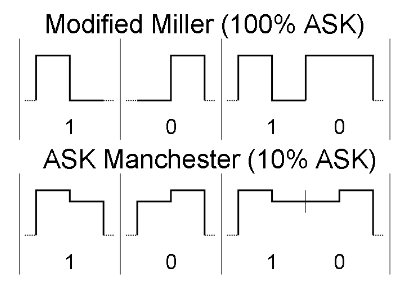
\includegraphics{kodolas}
	\caption{Módosított Miller (100\% ASK) és Manchester (10\% ASK) kódolások}		\label{fig:kodolas}
\end{figure}

\subsection{Biztonsági vonások}
Először is fontos megjegyezni, hogy az alacsony működési távolság, amely az \emph{NFC}-t
jellemzi, annak ellenére nem biztosítja a biztonságos kommunikációt, hogy tudatos
felhasználói interakciót igényel.

Különböző lehetőségek állnak rendelkezésre az \emph{NFC} technológia megtámadására.
Egyrészről az eszközöket fizikailag is lehet manipulálni. Ez jelentheti az \emph{NFC}
\emph{tag} (címke) eltávolítását, vagy fémfóliával bevonását, mellyel árnyékolni lehet
a rádióhullámokat.

Amennyiben egy tagen érzékeny információk találhatóak, annyiban a taget meg kell
védeni a  jogtalan olvasástól és írástól. Természetesen a csak olvasható tagek
védettek a jogtalan írás ellen.

A hibaérzékelésre az \emph{NFC} a ciklikus redundancia vizsgálatot (CRC) használja.
Ezzel az eszköz képes érzékelni, hogy a megkapott adat sérült-e. 

A továbbiakban különböző lehetséges \emph{NFC} támadásokat fogok vizsgálni. A legtöbb
ilyen támadásra létezik védekezési megoldás, amellyel csökkenteni, vagy akár 
meg is lehet szüntetni a veszélyforrást. A következőkben nagyban támaszkodok
Haselsteiner és Breitfuss: \emph{Security in Near Field Communication}
\cite{nemetbiztonsagnfc} művére.


\subsubsection{Lehallgatás}
Az \emph{NFC}, mint minden rádióhullámokat használó technológia, nem véd a lehallgatás
ellen. A támadó a megfelelő antennával és tudással le tudja hallgatni a 
vezetéknélküli kommunikációt. A legfőbb probléma a lehallgatás esetén az, 
hogy közel kell lenni a kommunikáló eszközökhöz. Az, hogy mennyire közel kell
lennie a támadónak a lehallgatáshoz sok paramétertől függ, mint az antenna 
geometriája, a küldés energiaszintje, a támadó és dekódoló eszközök minősége, stb.
Ezen felül érdemes kiemelni, hogy a lehallgatás távolsága nagyban függ a működés
módjától is: aktív módban akár 10 méteres távolságból is le lehet hallgatni, 
passzív módban pedig legfeljebb 1 méter lehet a lehallgatás távolsága.

Ez ellen a biztonságos csatorna kiépítése az egyedüli védekezési technika, 
amely sok más támadás ellen is egy lehetséges védekezési mód.

\subsubsection{Adattörlés}
Megfelelő közelben a támadó képes lehet az átvitt adat törlésére, érthetetlenné
tételére. Ehhez szüksége van a moduláció és a kódolás ismeretére. Ezek ismeretében
képes a vivőfrekvencián a megfelelő időben kiadott ellenkező fázisú kioltó jel
kiadására. 

Az adattörlés ellen aktív figyeléssel lehet védekezni, hiszen a jel elrontásához
egy nagyságrenddel több energia szükséges.

\subsubsection{Adatmódosítás}
Adatmódosítás esetén nagyon másképp kell eljárni a különböző modulációk esetén.
Amennyiben 100\%-os ASK-t használunk, annyiban amikor alacsony a jelszint, akkor
kell sugározni, és amikor normálisan magas lenne a jelszint, akkor egy olyan 
jelet kell kiadni, ami pontosan kioltja az eredeti jelet. Az előbbi könnyen 
megvalósítható, az utóbbi gyakorlatilag lehetetlen. Ha megvizsgáljuk 
\aref{fig:kodolas}-es ábrát, láthatjuk, hogy a kitöltéssel az 11-es bitpárt
lehet 10-ra módosítani Miller kódolás esetén.

10\%-os ASK esetén azonban minden bit megváltoztatható, hiszen a vevő csak a 
jelek egymáshoz viszonyított relatív erősségét vizsgálja (természetesen egy
engedélyezett amplitúdó intervallumon belül). Ekkor ha az alacsony jelszinthez 
annyit adunk, hogy az arányok felcserélődjenek, akkor ellentétes bit vételét
érhetjük el.

Az adattörléshez hasonlóan itt is a csatorna ellenőrzésével lehet észrevenni,
ha valaki megváltoztatja a jelarányokat.

\subsubsection{Adatbeszúrás}
Ehhez arra van szükség, hogy a célpont eszköz lassan küldje ki a válaszát, 
valamilyen okból kifolyólag. A támadó azelőtt küldhet extra információt, mielőtt
az eredeti célpont átküldené a válaszát, de amint az eredeti célpont elindítja a
választ, és a támadó még nem fejezte be az adat beszúrást, annyiban összeütközés
jön létre, így a kezdeményező mindkettő választ eldobja.

\subsubsection{Man-in-the-Middle}
A klasszikus Man-in-the-Middle támadás esetében már akkor elbukhat
a támadás, ha a beékelődő támadó zavarja a célpontnak küldött jelet, de az
érzékeli a zavarást. Ha nem érzékeli, akkor is elbukhat később a támadás, 
hiszen a válasz esetén mind a támadó, mind az eredeti célpont egyszerre válaszol,
így a kezdeményező mindkettő üzenetet venni fogja és ütközés jön létre.
Aktív módban amikor a kezdeményező lekapcsolja a mezejét, akkor a támadó szabadon
küldhet, azonban ezt a jelet a kezdeményező is megkapja és a célpont válaszaként
próbálja értelmezni. Haselsteiner és Breitfuss meg is jegyzik, hogy ezek alapján
egy Man-in-the-Middle támadás sikerességének valószínűsége elhanyagolható.

Más támadásokkal, mint az átjátszással, vagy féregjárattal kombinált támadás
esetén viszont megnő a támadás sikerének valószínűsége.

\section{Az NFC és egyéb vezetéknélküli technológiák}
Az NFC korlátaival az egyszerű szemlélőnek feleslegesnek mutathatja a 
technológiát a többi vezetéknélküli technológia fényében, de előnyei 
(olcsóság, kapcsolat felépülésének sebessége)
nagyon alkalmassá teszi a többi technológiával való együtt használásra.

\subsection{RFID vs. NFC}
Az RFID (Radio Frequency IDentification) tulajdonképpen az NFC előfutára, ebből
fejlődött ki. Definíció szerint az RFID a rádióhullámos azonosításra használt technológia.

\subsubsection{Működési frekvencia}
Az RFID három különböző frekvenciaszinten képes működni, attól függően, hogy milyen 
távolságból való leolvasást szeretnénk használni:
\begin{itemize}
\item Alacsony frekvencia: 125-134 kHz, max. 10 cm távolságig,
\item Magas frekvencia: 13,56 MHz, max. 30 cm távolságig,
\item Ultra magas frekvencia: 856--960 MHz, akár 100 m távolságig.
\end{itemize}

Ezzel szemben az NFC csak a 13,56 Mhz-en működik, ugyanazon, mint a magas frekvenciás RFID.
Ez is mutatja a szoros kapcsolatukat és az NFC ilyen RFID tagekkel való kompatibilitását.

\subsubsection{Működési mód}
Ahogyan az NFC eszközök, úgy az RFID eszközök is lehetnek aktívak vagy passzívak, de 
az utóbbi esetén ez jelentősen megváltoztatja leolvasás távolságát: az aktív RFID
eszközök (ezek amelyek belső energiaforrással rendelkeznek) teszik lehetővé 
az akár 100 méteres távolságból történő leolvasást. Ezt tárgyak lokalizációra 
használják nagy raktárakban. Passzív módban, amikor nem rendelkezik saját
energiaforrással az eszköz, akkor csak 25 méter lehet a leolvasás maximum távolsága.
Ilyenkor az NFC-hez hasonlóan a leolvasó nyújtja az energiát.

\subsubsection{Felhasználási területek}
\begin{itemize}
\item
Az RFID jellemző felhasználási területei:
\begin{itemize}
\item Eszköznyilvántartás
\item Verseny időmérése
\item Raktárkészlet menedzsment
\item Eszköz követés
\item Hozzáférés-szabályozás
\item Belépőkapuk.
\end{itemize}

\item
Az NFC felhasználási területei:
\begin{itemize}
\item Információmegosztás mobil eszközök között
\item Érintésmentes fizetés (kártyával vagy mobiltelefonnal)
\item Okos poszterek: NFC képes mobiltelefonnal exkluzív tartalom elérése.
\end{itemize}
\end{itemize}

\subsection{Bluetooth vs. NFC}
Alapvetően az NFC rövidebb kapcsolatra lett kialakítva, amikor a két eszköz közel 
található egymáshoz. Nincs szükség külön párosításra. A Bluetooth-nak szüksége 
van párosításra, de stabilabb és hosszabb időtartamon keresztül fenntartandó
kapcsolatok kiépítésére szolgál.

Az NFC és a Bluetooth egymásnak nem versenytársai, hanem kiegészítő technológiái.

Egy Bluetooth eszköz mindenképpen igényel külső energiaforrást. Az NFC-nél láttuk, 
hogy nem ez a helyzet.

A kapcsolat felépülését tekintve az NFC sokkal gyorsabb a Bluetooth-nál: nem igényel
többet csak a két eszköz összeérintését, míg a Bluetooth-nál szükség van kód
cserére, ami az NFC azonnali kapcsolatkiépítésével szemben hosszú másodpercekbe
telik. Átviteli sebességnél azonban jóval magasabb sebességet lehet elérni
Bluetooth-tal. Amíg az NFC csak néhány száz kbit/s-os sebességre képes, addig
a Bluetooth-tal néhány Mb/s-ot is el lehet érni. A Bluetooth a 2,4 GHz-es 
frekvenciasávban működik, ez által akár 100 méteres hatótávolsággal is 
rendelkezhet.

Ezek a különbségek okozzák a teljesen más felhasználási módokat is. Az NFC-vel 
szemben a Bluetooth adatátvitelre, perifériák működtetésére, vezeték nélküli 
hálózatok kiépítésére használható.

\section{Összefoglalás}
Láthattuk, hogy az NFC nem egy teljesen újszerű technológia, hanem már létezőek jó
tulajdonságait felhasználva kialakított vezeték nélküli kommunikációs mód.
Nagy népszerűségét olcsóságának köszönheti és annak, hogy a szolgáltatók 
rájöttek, hogy mennyire könnyen kapcsolhatnak ehhez a technológiához olyan
szolgáltatásokat, amellyel könnyen lehet pénzt keresni, elég csak a mobilos
fizetésre gondolni, amely nem olyan régen indult el Magyarországon is.
Nagy az iparágat befolyásoló világvállalatok is látnak benne jövőt (Apple, Google),
így várhatóan az elterjedtsége az elkövetkezendő években folyamatosan növekedni fog.

\begin{thebibliography}{9}

\bibitem{elektromagnesesterek}
    Dr. Zombory László,
    \emph{Elektromágneses terek},
    Műszaki kiadó, Budapest,
    2008.
  
\bibitem{biztonsagnfc}
    Solt Benedek Pál,
    \emph{Biztonság a Near Field Communication szabványaiban},
    2010.11, 
    http://www.hit.bme.hu/~buttyan/courses/BMEVIHIM219/2010/HF-reports/SoltBenedek.pdf
    
\bibitem{nemetbiztonsagnfc}
    Ernst Haselsteiner, Klemens Breitfuss,
    \emph{Security in Near Field Communication (NFC)},
    2006. július,
    
    http://events.iaik.tugraz.at/RFIDSec06/Program/papers/002\%20-\%20Security\%20in\%20NFC.pdf
    
\bibitem{nfc1}
    ISO 2004, ISO/IEC  18092-4., 
    \emph{Near Field Communication Interface and Protocol (NFCIP-1)}

\bibitem{nfc2}
    ISO 2005, ISO/IEC  21481.,
    \emph{Near Field Communication Interface and Protocol-2 (NFCIP-2)}
    
\bibitem{rfid}
    James Thrasher,
    \emph{RFID vs. NFC},
    2013. 10. 11.
    
    http://blog.atlasrfidstore.com/rfid-vs-nfc
    
\bibitem{bluetooth}
    Mrinal Saha,
    \emph{What is the Difference Between NFC and Bluetooth?}
    
    2015. 07. 07., http://hubpages.com/technology/nfc-vs-bluetooth

\end{thebibliography}

\end{document}
